\usetikzlibrary{decorations.pathreplacing}
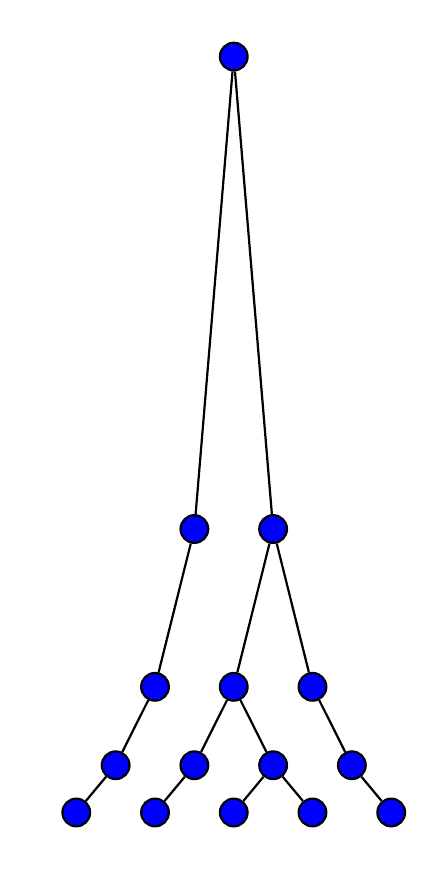
\begin{tikzpicture}
    \begin{scope}[auto, every node/.style={draw=black,circle,thick,minimum size=1em,fill=blue}]
        \node (A_1) at (1, 0) {};
        \node (A_2) at (2, 0) {};
        \node (A_3) at (3, 0) {};
        \node (A_4) at (4, 0) {};
        \node (A_5) at (5, 0) {};

        \node (B_1) at (1.5, 0.5*1.2) {};  % N = 5, 5 choose 2 = 10, 5 / 10 = 0.5
        \node (B_2) at (2.5, 0.5*1.2) {};
        \node (B_3) at (3.5, 0.5*1.2) {};
        \node (B_4) at (4.5, 0.5*1.2) {};

        \node (C_1) at (2, 1.33*1.2) {};  % N = 5, 4 choose 2 = 6, 5 / 6 = 0.83
        \node (C_2) at (3, 1.33*1.2) {};
        \node (C_3) at (4, 1.33*1.2) {};

        \node (D_1) at (2.5, 3*1.2) {};  % N = 5, 3 choose 2 = 3, 5 / 3 = 1.66
        \node (D_2) at (3.5, 3*1.2) {};

        \node (E_1) at (3, 8*1.2) {};  % N = 5, 2 choose 2 = 1, 5 = 5
    \end{scope}

    \begin{scope}[every edge/.style={draw=black,thick}]
        \path (A_1) edge (B_1);
        \path (A_2) edge (B_2);
        \path (A_3) edge (B_3);
        \path (A_4) edge (B_3);
        \path (A_5) edge (B_4);

        \path (B_1) edge (C_1);
        \path (B_2) edge (C_2);
        \path (B_3) edge (C_2);
        \path (B_4) edge (C_3);

        \path (C_1) edge (D_1);
        \path (C_2) edge (D_2);
        \path (C_3) edge (D_2);

        \path (D_1) edge (E_1);
        \path (D_2) edge (E_1);
    \end{scope}

    \node (T_A) at (0.5, -0.25) {};
    \node (T_B) at (0.5, 0.6+0.25) {};

    \node (T_B2) at (0.5, 0.6) {};
    \node (T_C) at (0.5, 1.6+0.25) {};

    \node (T_C2) at (0.5, 1.6) {};
    \node (T_D) at (0.5, 3.6+0.25) {};

    \node (T_D2) at (0.5, 3.6) {};
    \node (T_E) at (0.5, 9.6+0.25) {};
\end{tikzpicture}